\documentclass[12pt]{article}

% \usepackage{report}



\usepackage{float}

\usepackage[margin=2cm]{geometry}
% \usepackage{romannum}
\usepackage{blindtext}
\usepackage{multirow}
\usepackage{graphicx}
\usepackage{nopageno}
\usepackage{graphicx}

\begin{document}
\date{}{}
\title
{
    \vspace{150pt}
    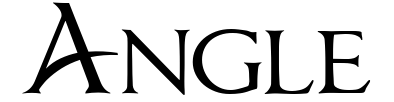
\includegraphics[scale=0.7]{./images/final_angle.png}
{\LARGE{\\ Language Specification}}
}

\author{
    \vspace{140pt}\\
Group 7                                     \\
Tejal Kulkarni           -  CS21BTECH11058  \\
Deepshikha               -  CS21BTECH11016  \\
Nitya  Bhamidipaty       -  CS21BTECH11041  \\ 
Muskan Jaiswal           -  CS21BTECH11037 
}
\maketitle
\pagebreak
\tableofcontents
\pagebreak
\section{Motivation}
The motivation behind designing this language is to combine computation and geometry.
Though there are other software for creating diagrams, they do not natively support programming.
The idea is to make abstract concepts more intuitive by easing the process of making geometrical figures.
We feel that this language will help automate the process of visualizing geometrical figures.
An user can integrate external data with code to create diagrams.
Our language is mainly intended for high school geometry. 
We feel that integrating our language with school curriculum can help nurture programming mindset at a young age. 
We hope that our language can be extended further to become the latex of geometry.

\section{Lexical Convention}

\subsection{Comments}
Both single and multi-line comments are supported
\begin{verbatim}
    $ single-line comment 
    $$ 
        multi-line comment 
    $$
\end{verbatim}
Nested comments are not allowed.
\begin{verbatim}
    $$ not a $$valid comment$$ $$
\end{verbatim}

\subsection{Whitespace}
All whitespaces are ignored except in places where white space are required for separation of tokens.
In 'Angle', each statement is terminate by a new line or EOF.

\subsection{Identifiers}
The rules for identifiers is the same as in C/C++.
It starts with letter or underscore, followed by letters, digits or underscores. Our language is case-sensitive.

\subsection{Reserved Keywords}
\begin{center}
\begin{tabular}{ | c | c | c| c | c |c|c|c|c|} 
  \hline
  if & elif & else & repeat & until & int  & real & label & point \\ 
  \hline
   bool & line & circle & tri & para & regPoly & and & or & not\\ 
  \hline
  func & stop & advance & return & true & false & fig & void & angle\\
  \hline
  
\end{tabular}
\end{center}


\section{Data Types}

\subsection{Primitive Data Types}
\begin{center}
\begin{tabular}{ | c | c | c| c | c |c|} 
  \hline
  Data Types & Description \\ 
  \hline
  int & 32-bit signed integer value \\
 real & 64-bit signed floating point number \\
 label & sequence of characters (string) \\
 bool & stores true/false value\\
 point &  coordinates of a point  \\
angle & angle between three points in degrees \\
\hline
\end{tabular}
\end{center}

\subsection{Non-primitive Data Types}

\begin{center}
\begin{tabular}{ | c | c |} 
  \hline
  Data Types & Description \\ 
  \hline
  array & sequence of primitive/non-primitive data types  \\
line & line joining two points \\
circle & circle with a center and radius \\
tri & triangle  \\
para & parallelogram  \\
regPoly & regular polygon \\
\hline
\end{tabular}
\end{center}


\section{Declarations}
Program consists of various entities such as variables, function and figures. Each of these entities must be declared before use.

\subsection{Variable declaration}
\subsubsection{Primitive}
\begin{verbatim}
    int a = 0
    real a = 4.5
    label s = "Angle"            $ Should use ""
    bool x = true
    point p = (2,3,"A")          $ (x-coord, y-coord, label) 
    angle a = < p q r >          $ by default , display is true 
    angle b = < p q r , false >  $ false implies not to be displayed 
\end{verbatim}

\subsubsection{Non-Primitive}
\begin{verbatim}
     $$ ARRAY $$
        int a[4] := {1,2,3,4}     $ array declaration 
\end{verbatim}
\pagebreak
\begin{verbatim}
     $$ LINE $$
         line l := p-q             $ line declaration where p,q are points 
         line l[] := p<->q-r->s    $ line array declaration 
         $$
            <-> : denotes line
            -   : denotes segment
             -> : denotes vector
         $$


    $$ CIRCLE $$
        circle c := Circle(p,r)    $ (centre,radius)

    $$ TRIANGLE $$
        tri t := Tri(p,q,r)        $ three points declaration
        tri t := Tri(4,8,5)        $ SSS declaration
        tri t := Tri(5,4)          
        $$ 
            RHS declaration :
                first argument is hypotenuse 
                second is one of the other side
        $$
    
    $$ PARALLELOGRAM $$
        para p := Para(3,60,8)     $ SAS declaration
        $ 2 adjacent sides and the angle contained by them

    $$ REGULAR POLYGON $$
        regPoly r := RegPoly(3,8)  $ (no of sides , length of sides)
   
\end{verbatim}

\subsection{Declaration Scope}
In our language, an identifier in global scope can be redefined in any other scope including functions and figures. An identifier defined in a scope cannot be redefined within the same scope.

% \subsection{Array declaration}
% \begin{verbatim}
%     int a[4] = {1,2,3,4}
%     line l[] = p<->q-r->s where p,q,r,s are points.
%     <-> : denotes line
%     -   : denotes segment
%     ->  : denotes vector
% \end{verbatim}

\subsection{Function declaration}

default values

A function like in other programming languages can be used to modularize your code and can be called anywhere in the global scope or figures (described in the next section).
\begin{verbatim}
    func return_type function_name(argument_list) {
        $ statements
    }
\end{verbatim}
If function return type is not void then you must include return statement in the function.
\subsection{Figure declaration}
Figure consists of a set of geometrical objects that could be displayed with a given scale and center. Scale is the size of the figure and center is the origin for the objects part of that figure. Functions can be called inside figures as well.
\begin{verbatim}
    fig figure_name(scale,center) {
       $ statements
    }
\end{verbatim}
Example use of figures:
\begin{verbatim}
    $ Creates a series of kites
    
    fig kite (scale := 1, center := (0, 0)){

        para k := Para(5, 60, 5)
        k.DIAGONAL()
        
    }

    int N := 4 $ No of kites
    
    repeat (int i := 1|i <= N|i++)
    {
        kite(1, (0, i))
    }
\end{verbatim}
% \subsection{Initialisers}


\section{Operators}
\subsection{Compatible Types +}
\begin{itemize}
    \item POINT
    \item LABEL
    \item REAL, BOOL, INT, ANGLE are arithCompatible
\end{itemize}


We have two new operators , parallel ($\parallel$) and perpendicular ( $|-$ ) .
\begin{verbatim}
    p || q              
    $ check if lines p and q are parallel, returns boolean value 

    p |- q
    $ check if lines p and q are perpendicular, returns boolean value 
\end{verbatim}
Example:
\begin{verbatim}
    line l1, l2, l3 

    $ Can have multiple lines aswell
    if (l1 || l2 || l3)
        return 0;
        
\end{verbatim}
\subsection{Precedence}
\begin{center}
\begin{tabular}{ | c | c | c| c | c |} 
  \hline
  Operator & Symbol & Associativity \\ 
  \hline
Parenthesis & ( ) & left to right  \\
Member access & . & left to right \\
Unary Negation & not & right to left  \\
Increment & ++ & right to left  \\
Decrement & -- & right to left  \\
Exponent & ${}^\wedge$ & left to right  \\
% Modulo & \% & left to right & \\
Multiplication,Division,Modulo & *,/,\% & left to right  \\
Addition,Subtraction & +,- & left to right  \\
Relational & $<=$,$>=$,$<$,$>$,==,!= & left to right  \\
Logical & and,or & left to right  \\
Parallel & $\parallel$ & left to right  \\
Perpendicular & $|-$ & left to right  \\
Assignment  & :=,+:=,-:=,${}^\wedge$:=,/:=,\%:= & right to left  \\
\hline
\end{tabular}
\end{center}

\section{Statements}

\subsection{Compound Statements}
A compound statement is a sequence of statements enclosed by braces, for example:
\begin{verbatim}
    {
       int a := 9
       line l := p-q
    }
\end{verbatim}

\subsection{Control Flow}

\subsubsection{Conditionals}
\begin{verbatim}
$ if - elif - else
    if (i <= 3){        
        $ stmt
    }
    elif (i > 3){
        $ stmt
    }
    else{
        $ stmt
    }
\end{verbatim}
\pagebreak
\begin{verbatim}
$ if - else
    if (i <= 3){    
        $ stmt
    }
    else{
        $ stmt
    }
$ single statement if
    if (i <= 3)        
        $ stmt    
\end{verbatim}

\subsubsection{Loop Statements}
\begin{verbatim}
    $$ SIMILAR TO FOR LOOP $$
    repeat(int i := 0 | i < n | i++ )
    {
       $ statemtents
        advance        $ continue statement
    }

    $$ SIMILAR TO WHILE LOOP $$
    until(i < l)
    { 
       $ statements
        stop           $ break statement
    }
\end{verbatim}

\section{Built-in and Standard Library functions}

We plan to implement some standard libraries to provide support for the following domains. Some examples are shown below.
\begin{itemize}
    \item Line 
\begin{verbatim}
    point p := INTERSECTION(a,b)           $ a and b are lines
    point p := MIDPOINT(l)                 $ l is a line segment
    point p := MIDPOINT(a,b)               $ a, b are points
    real dist := SHORTEST_DISTANCE(a,b)    $ a, b are points
    line p := ANGLE_BISECTOR(a,b)          $ a, b are lines
    line p := LINE_AT_ANGLE(40,a,q)        $ (angle,line,point)
\end{verbatim}
\item Circle
\begin{verbatim}
    $ o:center, r:radius
    circle c := Circle(o,r)                 
    $ q is point of contact of line p to circle c
    line p := c.TANGENT(q)  
    $ c1 and c2 are circles               
    point p[] := INTERSECTION(c1,c2)   
    line l[] := COMMON_TANGENT(c1,c2)
\end{verbatim}

\item Triangle
\begin{verbatim}
    tri t := Tri(a,b,c)
    point p := t.CIRCUMCENTRE()
    $ excentre opposite to point q of the triangle t
    point p := t.EXCENTRE(q) 
    point p := t.INCENTRE()    
    point p := t.ORTHOCENTRE() 
    $ q is point of triangle from which altitude is drawn  
    line l := t.ALTITUDE(q)
    $ q is vertex of triangle from which median is drawn  
    line l := t.MEDIAN(q)
    point p := t.CENTROID()            
\end{verbatim}

\item Parallelogram
\begin{verbatim}
    para p := Para(a,40,b)
    line l[] := p.DIAGONAL()
\end{verbatim}
\item Regular Polygon
\begin{verbatim}
    regPoly h := regPoly(3, 6)
    h.AREA()
    h.PERIMETER()
\end{verbatim}
\item We have two member functions, area and perimeter for all 2D geometric objects.
\begin{verbatim}
    || p ||         $ distance between p and origin
    || p - q ||     $ distance between p and q 
\end{verbatim}
\end{itemize}

\section{Sample program}
\begin{verbatim}
func fact(int n){
    if (n == 1 or n == 0){
        return 1
    }
    else{
       return (fact(n-1)*n)
    }
}
\end{verbatim}
\pagebreak
\begin{verbatim}
$ Figure to display the circumcircle of a triangle
fig figure_1 (1,(0,0)){
    point a := (1,2)
    point b := (2,7)
    point c := (7,1)
    tri t := Tri(a,b,c)
    point o := t.CIRCUMCENTRE()
    real r := || a-o ||
    circle c := (o,r)   
}

$ Figure to display a parallelogram and its diagonals and print its area
fig figure_2 (1,(2,0)){
    para p := Para(3,60,8)
    real area := p.AREA()
    print(area)
}

$ Figure to display adjacent circles with radius equal to sequence of factorials
fig figure_3(scale := 2, centre := (0,0)){
    point p := (0,0)
    int n := 3
    repeat(int i := 1 | i <= n | i++ ){
        Circle(p,fact(i))
        p.x := p.x + 1
    }
}

$ Syntax to display figures$
figure_1()
figure_2()
figure_3()
\end{verbatim}



\end{document}